% Standalone source of the figure fig:twocentre of the coupling-integrals paper.
% Build: pdflatex fig_twocentre.tex; the paper includes the PDF. Grey scale only: line styles, not colour.
\documentclass[border=2pt]{standalone}
% Shared preamble of the standalone figures of the coupling-integrals paper.
\usepackage{amsmath,amssymb,bm}
\usepackage{tikz}
\usetikzlibrary{calc,arrows.meta}
\newcommand{\bR}{\mathbf{R}}
\newcommand{\bs}{\mathbf{s}}
\newcommand{\bu}{\mathbf{u}}
\newcommand{\bx}{\mathbf{x}}

\begin{document}
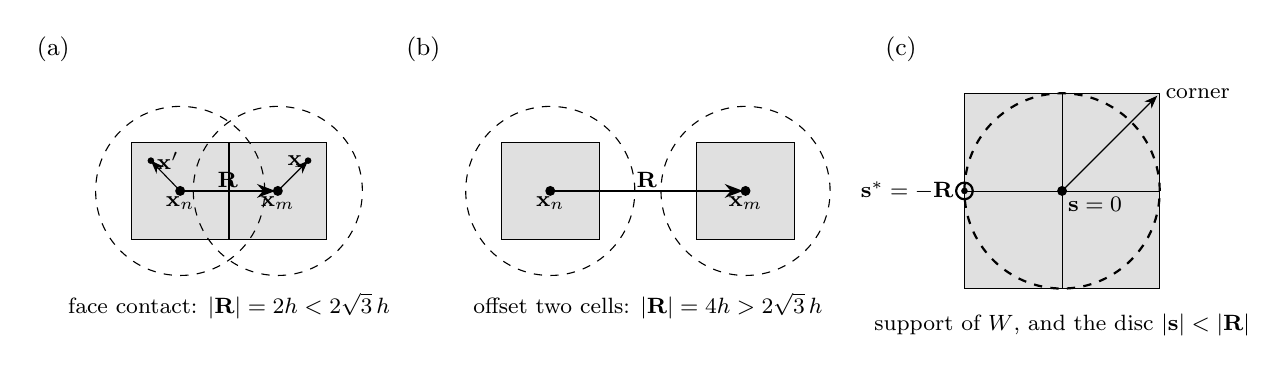
\begin{tikzpicture}[>=Stealth, x=0.62cm, y=0.62cm, font=\small]
  % ---------------------------------------------------------------- (a) two cells that touch
  \begin{scope}
    \node at (-2.6,2.9) {(a)};
    \fill[black!12] (-1,-1) rectangle (1,1);
    \fill[black!12] (1,-1) rectangle (3,1);
    \draw (-1,-1) rectangle (1,1);
    \draw (1,-1) rectangle (3,1);
    \draw[dashed] (0,0) circle (1.732);
    \draw[dashed] (2,0) circle (1.732);
    \fill (0,0) circle (1.8pt) node[below, font=\footnotesize, inner sep=2pt] {$\bx_n$};
    \fill (2,0) circle (1.8pt) node[below, font=\footnotesize, inner sep=2pt] {$\bx_m$};
    \draw[->, thick] (0,0) -- node[above, font=\footnotesize, inner sep=1pt] {$\bR$} (1.95,0);
    % a source point and a field point, at u' and u from the centres
    \draw[->] (0,0) -- (-0.6,0.62);
    \fill (-0.6,0.62) circle (1.2pt) node[right, font=\footnotesize, inner sep=2pt] {$\bx'$};
    \draw[->] (2,0) -- (2.62,0.62);
    \fill (2.62,0.62) circle (1.2pt) node[left, font=\footnotesize, inner sep=2pt] {$\bx$};
    \node[font=\footnotesize] at (1,-2.35) {face contact: $|\bR|=2h<2\sqrt3\,h$};
  \end{scope}
  % ---------------------------------------------------------------- (b) two cells two widths apart
  \begin{scope}[xshift=4.7cm]
    \node at (-2.6,2.9) {(b)};
    \fill[black!12] (-1,-1) rectangle (1,1);
    \fill[black!12] (3,-1) rectangle (5,1);
    \draw (-1,-1) rectangle (1,1);
    \draw (3,-1) rectangle (5,1);
    \draw[dashed] (0,0) circle (1.732);
    \draw[dashed] (4,0) circle (1.732);
    \fill (0,0) circle (1.8pt) node[below, font=\footnotesize, inner sep=2pt] {$\bx_n$};
    \fill (4,0) circle (1.8pt) node[below, font=\footnotesize, inner sep=2pt] {$\bx_m$};
    \draw[->, thick] (0,0) -- node[above, font=\footnotesize, inner sep=1pt] {$\bR$} (3.95,0);
    \node[font=\footnotesize] at (2,-2.35) {offset two cells: $|\bR|=4h>2\sqrt3\,h$};
  \end{scope}
  % ---------------------------------------------------------------- (c) the separation s, face contact
  \begin{scope}[xshift=11.2cm]
    \node at (-3.3,2.9) {(c)};
    % the support of W: |s_i| <= 2h, with its eight pieces
    \fill[black!12] (-2,-2) rectangle (2,2);
    \draw (-2,-2) rectangle (2,2);
    \draw[very thin] (0,-2) -- (0,2);
    \draw[very thin] (-2,0) -- (2,0);
    % the disc |s| < |R| on which the Taylor series of P(R + s) about s = 0 converges
    \draw[thick, dashed] (0,0) circle (2);
    \fill (0,0) circle (1.8pt) node[below right, font=\footnotesize, inner sep=2pt] {$\bs=0$};
    % the singular point s* = -R, on the boundary of the support
    \draw[thick] (-2,0) circle (3pt);
    \fill (-2,0) circle (1.2pt);
    \node[left, font=\footnotesize, inner sep=2pt] at (-2.1,0) {$\bs^*=-\bR$};
    % a corner of the support, outside the disc
    \draw[->] (0,0) -- (1.95,1.95);
    \node[right, font=\footnotesize, inner sep=2pt] at (2,2) {corner};
    \node[font=\footnotesize, align=center] at (0,-2.75) {support of $W$, and the disc $|\bs|<|\bR|$};
  \end{scope}
\end{tikzpicture}
\end{document}
